\documentclass[12pt]{article}
\usepackage[margin=1in]{geometry}
\usepackage{setspace}
\onehalfspacing

% Start of preamble
%==========================================================================================%
% Required to support mathematical unicode
\usepackage[warnunknown, fasterrors, mathletters]{ucs}
\usepackage[utf8x]{inputenc}

\usepackage[dvipsnames,table,xcdraw]{xcolor}

% Standard mathematical typesetting packages
\usepackage{amsmath,amssymb,amscd,amsthm,amsxtra}
\usepackage{mathtools,mathrsfs,xparse,newtxtext,newtxmath}

% Symbol and utility packages
\usepackage{cancel, textcomp}
\usepackage[mathscr]{euscript}
\usepackage[nointegrals]{wasysym}
\usepackage{apacite}

% Extras
\usepackage{physics}  
\usepackage{tikz-cd} 
\usepackage{microtype}
\usepackage{enumitem}
\usepackage{titling}
\usepackage{graphicx}

% Common shortcuts
\def\mbb#1{\mathbb{#1}}
\def\mfk#1{\mathfrak{#1}}

\def\bN{\mbb{N}}
\def \C{\mbb{C}}
\def \R{\mbb{R}}
\def\bQ{\mbb{Q}}
\def\bZ{\mbb{Z}}
\def \cph{\varphi}
\renewcommand{\th}{\theta}
\def \ve{\varepsilon}
\newcommand{\mg}[1]{\| #1 \|}

% Often helpful macros
\newcommand{\floor}[1]{\left\lfloor#1\right\rfloor}
\newcommand{\ceil}[1]{\left\lceil#1\right\rceil}
\renewcommand{\qed}{\hfill\qedsymbol}
\renewcommand{\P}{\mathbb P\qty}
\newcommand{\E}{\mathbb{E}\qty}
\newcommand{\Cov}{\mathrm{Cov}\qty}
\newcommand{\Var}{\mathrm{Var}\qty}

% Sets
\usepackage{braket}

\graphicspath{{/}}
\usepackage{float}

\newcommand{\SET}[1]{\Set{\mskip-\medmuskip #1 \mskip-\medmuskip}}

% End of preamble
%==========================================================================================%

% Start of commands specific to this file
%==========================================================================================%

\usepackage{listings}  % For lstlisting environment
\usepackage{xcolor}    % For syntax highlighting (optional)

\lstset{
    basicstyle=\ttfamily\small,
    keywordstyle=\color{blue},
    commentstyle=\color{green},
    stringstyle=\color{red},
    numbers=left,
    numberstyle=\tiny\color{gray},
    breaklines=true,
    frame=single,
    language=Python
}

%==========================================================================================%
% End of commands specific to this file

\title{CSE 422 HW6}
\date{\today}
\author{Rohan Mukherjee}

\begin{document}
    \maketitle
    \subsection*{Problem 1.}
    \begin{enumerate}[label=(\alph*)]
        \item $k/n$ is exactly 0.21. We have 1200 pixels and 252 of them are not black.
        \item The linear program is the following:
        \begin{align*}
            \min \ & \sum_i y_i \\
            \text{s.t.} \ & A_r x = b_r, \\
                          & y \geq x, \\
                          & y \geq -x.
        \end{align*} 
        Introducing this auxilary variable $y$ is just so we can minimize the sum of $|x_i|$ as an LP. Of course, this is equivalent to the following LP:
        \begin{align*}
            \min \ & \sum_i |x_i| \\
            \text{s.t.} \ & A_r x = b_r.
        \end{align*}    
        I have checked that $x_{700} = x$ up to numerical precision ($10^{-6}$).
        \item Using binary search, I found $r^*$, the smallest $r$ so that $|x - x_r| < 0.001$, to be 658.

        \item Here is the plot of $\mg{x_i-x}$ for $i = r-10, \ldots, r+2$:
        \begin{figure}[H]
            \centering
            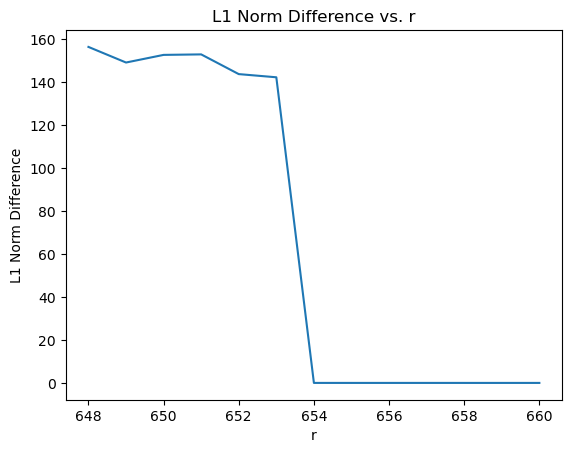
\includegraphics[width=0.7\textwidth]{sharp_dropoff.png}
        \end{figure}
        There is very clearly a giant cliff at $654$. This is quite surprising! From around a value of 160 to like almost 0.

        \item $\hat r(0.5) = 627$ for me. 
        \item As a function of $p$, $\hat r(p)$ is as follows:
        \begin{figure}[H]
            \centering
            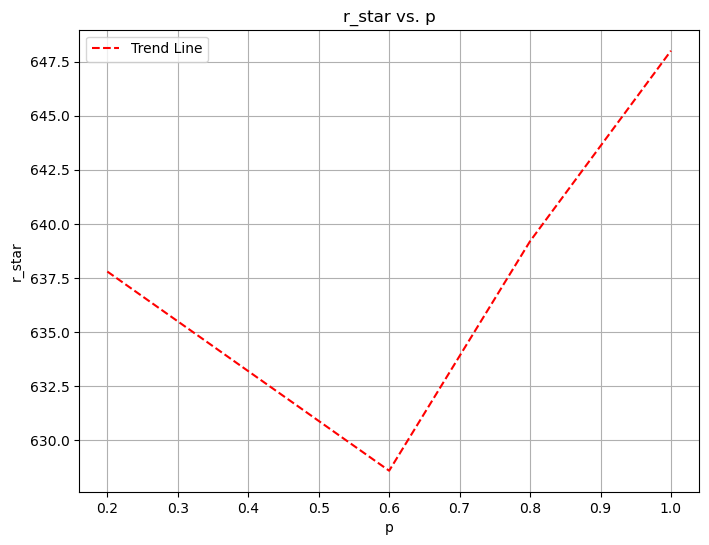
\includegraphics[width=0.7\textwidth]{r_hat.png}
        \end{figure}

        \item as a function of $p$, $\hat r(p)$ decreases until $0.6$, then starts increasing again. Smaller values of $p$, such as 0.2, would cause 80\% of entries to be 0. Then the matrix would be very sparse. Then every operation on a sparse matrix is quicker. Products, describing separating hyperplanes, powers, etc. So I believe any of the methods we learned in class, the iterative ones or ellipsoid would just run a lot faster than if it had a lot of elements. I believe if you have too few elements, such as $p \to 0$, then the matrix would just look more and more like all 0s, and it wouldn't have enough dimensionality to accurately represent the data when we do $A_rx = b_r$. On the other hand, when there are no 0s, the process is significantly slower as we have to check every element, and as we have seen before almost all the vectors are tightly concentrated into 4 corners of a giant hypercube. This might lead to a nullspace with small sparsity, causing the method to outright fail. When we introduce some 0s, it has a lot more variety, since it can be in the middle of the hypercube too and we get good separation. So to avoid these two issues, it attains a min in the middle. 

        \item The restricted isometry condition is formulated as follows: 
        \begin{align*}
            (1-\ve)\mg{x}^2 \leq \mg{Ax}^2 \leq (1+\ve)\mg{x}^2.
        \end{align*}
        we proved this in class for suitably high dimension using johnson lindenstrauss lemma.
        
        For $X$ which is $\pm 1$ with equal probability, notice that (as $(2n)! \geq (2n)!! = 2^n n!$):
        \begin{align*}
            E(e^{\alpha X}) = \frac 12 (e^{\alpha} + e^{-\alpha}) = \frac 12 \sum_{n=0}^\infty \frac{\alpha^n + (-1)^n\alpha^n}{n!} = \sum_{n=0}^\infty \frac{\alpha^{2n}}{(2n)!} \leq \sum_{n=0}^\infty \frac{\alpha^{2n}}{2^n n!} = e^{\alpha^2/2}.
        \end{align*}
        Now we do literally magic. Let $Z$ be $N(0,1)$ independent of $X$. Then,
        \begin{align*}
            E(e^{\alpha Z}) = \frac{1}{\sqrt{2\pi}}\int_{-\infty}^\infty e^{\alpha t - t^2/2}dt = e^{\alpha^2/2} \frac{1}{\sqrt{2\pi}} \int_{-\infty}^{\infty} e^{-(t-\alpha)^2/2}dt = e^{\alpha^2/2}
        \end{align*}
        after a simple change of variables $u = t-\alpha$. From here, recall that if $X,Y$ are random variables then $E(\cph(X) \mid Y) = h(Y)$ where $h(y) = E(\cph(X) \mid Y = y)$. Since $X$ and $Z$ are independent $E(e^{\sqrt{2\lambda}XZ} \mid X = x) = E(e^{\sqrt{2\lambda} x Z})$ so $E(e^{\sqrt{2 \lambda } X Z} \mid X) = e^{\lambda X^2}$. Then clearly,
        \begin{align*}
            E(e^{\lambda X^2}) = E(E(e^{\sqrt{2 \lambda } X Z} \mid X)) = E(e^{\sqrt{2\lambda}XZ})
        \end{align*}
        Now we do the same trick, but conditioning on $Z$:
        \begin{align*}
            E(e^{\sqrt{2\lambda} XZ} \mid Z = z) = E(e^{\sqrt{2\lambda} X z}) \leq e^{\lambda z^2}.
        \end{align*}
        So $E(e^{\sqrt{2\lambda}XZ} \mid Z) \leq e^{\lambda Z^2}$. Thus we have concluded:
        \begin{align*}
            E(e^{\lambda X^2}) \leq E(e^{\lambda Z^2})
        \end{align*}
        Now, by letting $u = t\sqrt{1 - 2\lambda}$, with $dt = du/\sqrt{1-2\lambda}$, we get:
        \begin{align*}
            E(e^{\lambda Z^2}) = \frac{1}{\sqrt{2\pi}} \int_{-\infty}^{\infty} e^{t^2(-1/2 + \lambda)}dt = \frac{1}{\sqrt{2\pi(1-2\lambda)}}\int_{-\infty}^\infty e^{-u^2/2}du = \frac{1}{\sqrt{1 - 2\lambda}}.
        \end{align*}
        Then using the taylor expansion $\log(1-x) = -\sum_{k \geq 1} x^k/k$, and dropping the denominators,
        \begin{align*}
            \qty|\log E(e^{\lambda(Z^2-1)})| = \qty|-\lambda - \frac 12 \log(1-2\lambda)| \leq -\lambda + \frac 12 (2\lambda + (2\lambda)^2 + \cdots) = \frac{2\lambda^2}{1-2\lambda}
        \end{align*}
        Now, for $A \in \R^{k \times n}$ with $\SET{\pm 1/\sqrt n}$ uniform entries that are independent, fix a unit vector $u \in \R^n$. By definition, $\mg{Au} = \sum_{i=1}^k (a_i^Tu)^2$. Define $Y_i = a_i^Tu$. By Cauchy-Schwartz, $Y_i^2 \leq \frac 1n \sum X_j^2$ where $X_j = \sqrt{n}A_{ij}$ are independent and $\SET{\pm 1}$ random variables. Then since $e^x$ is increasing, by independence and Jensens inequality, noting $x^n$ is convex for $n \geq 1$, and using identically distributed, 
        \begin{align*}
            E(e^{\lambda (Y_i^2 - 1)}) \leq E(e^{\lambda \frac 1n (\sum X_j^2 - 1)}) = \prod E(e^{\frac \lambda n (X_j^2 - 1)}) \leq E(e^{\lambda (X^2 - 1)})
        \end{align*}
        Where $X$ is a $\pm 1$ random variable. By combining many past results, we have:
        \begin{align*}
            E(e^{\lambda (X^2 - 1)}) \leq e^{2\lambda^2/(1-2\lambda)}.
        \end{align*}
        We are ready to be done. Notice that:
        \begin{align*}
            P(\mg{Au}^2 \geq 1 + \ve) = P(e^{\lambda \sum_i Y_i^2 - 1} \geq e^{\ve \lambda k}) &\leq \frac{E(e^{\lambda \sum_i Y_i^2 - 1})}{e^{\ve \lambda k}} 
            \\&= \prod_i E(e^{\lambda (Y_i^2 - 1)})/e^{\ve \lambda k} \leq e^{2\lambda^2k/(1-2\lambda) - \ve \lambda k}.
        \end{align*}
        Choosing $\lambda = \ve/4$ shows that $P(\mg{Au}^2 > 1+\ve) \leq e^{-\ve^2k/8}$. The same argument shows it for $-\ve$, so $P(\mg{Au}^2 \in [1-\ve, 1+\ve]) \geq 1-2e^{-\ve^2k/8}$. For a prescribed probability $\delta$, choosing $k = \frac{24 \log 1/\delta}{\ve^2}$ suffices. 

        In fact, the same argument works for any random entries $X_{ij}$ with $E(e^{\alpha X_{ij}}) \leq e^{C\alpha^2}$ (with a slightly different constant).
    \end{enumerate}

    \subsection*{Problem 2.}
    \begin{enumerate}[label=(\alph*)]
        \item The naive reconstruction which I call $R$, where the original image is $I$, I defined by $R = I[i-1,j] + I[i+1,j] + I[i,j-1] + I[i,j+1] / Known[i-1,j] + Known[i+1,j] + Known[i,j-1] + Known[i,j+1]$. I have implemented this in the code. This gives the following image:
        \begin{figure}[H]
            \centering
            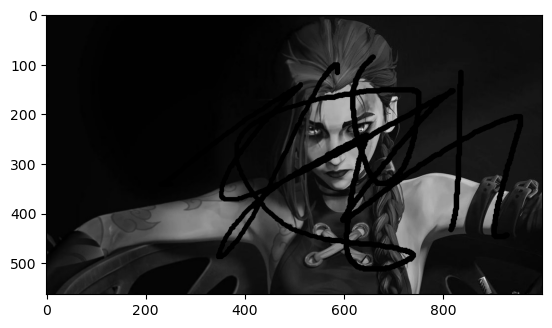
\includegraphics[width=0.7\textwidth]{naive_reconstruction.png}
        \end{figure}
        There are many reasons why this performs poorly. First off, the black line that has been drawn through the image has a thickness much greater than 4, so there are a lot of pixels who have no known neighbor. Second, it will add a slight blur to images with 4 known neighbors. It just doesn't really recover anything at all.

        My code is as follows:
        \begin{lstlisting}
reconstructed_image = np.copy(img)
for i in range(1, img.shape[0]-1):
    for j in range(1, img.shape[0]-1):
        reconstructed_image[i,j] = img[i-1, j] + img[i+1, j] + img[i,j-1] + img[i, j+1]
        number_known = Known[i-1, j] + Known[i+1, j] + Known[i,j-1] + Known[i, j+1]
        number_known = max(number_known, 1)
        reconstructed_image[i,j] /= number_known
        \end{lstlisting}

        \item I ran the linear program using total variation, and got the following image:
        \begin{figure}[H]
            \centering
            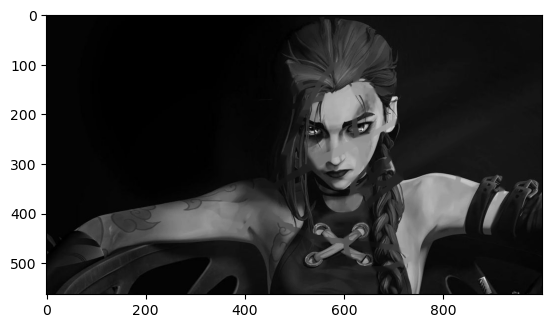
\includegraphics[width=0.7\textwidth]{tv_recovery.png}
        \end{figure}
        This is really good. It has gotten rid of the wide black line that was drawn through the image, however I can definitely see some distinct lines of varying color if you look close enough. Originally I had zoomed out and I literally thought it was the original image. But now I can see that the same lines from where the thick black one was originally are stil there, albeit with different, more natural colors. The naive reconstruction which really didn't do anything at all is very bad. This one is much better. The naive reconstruction looks a little brighter if you check out the far right side of the image. Also I have discovered that the tv reconstruction has gotten rid of part of her arm brace on the right side too. Overall, its quite good for what can be implemented so quickly.


        \item The documentation says $$\mathrm{tv}(X) = \sum_{i,j} \sqrt{(X_{i+1,j} - X_{i,j})^2 + (X_{i,j+1} - X_{i,j})^2}.$$
        For a fixed pair of $(i,j)$, if we let $Y^X_{i,j} = \begin{pmatrix} X_{i+1,j} - X_{i,j} \\ X_{i,j+1} - X_{i,j} \end{pmatrix}$, then $i,j$ term of this sum is just $\|Y^X_{i,j}\|_2$. Then for any other matrix $Z$, the $(i,j)$ term of $\mathrm{tv}(tX + (1-t)Z)$ is just $$\|tY^X_{i,j} + (1-t)Y^Z_{i,j}\| \leq t\|Y^X_{i,j}\| + (1-t)\|Y^Z_{i,j}\|.$$ since any norm is convex (this follows by triangle inequality and $\|\lambda x\| = |\lambda| \|x\|$.) Applying this for every term in the sum, and using linearity shows that $\mathrm{tv}(tX + (1-t)Z) \leq t\mathrm{tv}(X) + (1-t)\mathrm{tv}(Z)$.

        \item The full LP is as follows:
        \begin{align*}
        &\min \sum_{i,j} \sqrt{(X_{i+1,j}-X_{i,j})^2 + (X_{i,j+1}-X_{i,j})^2} \\
        &\text{s.t. } X_{i,j} = \mathrm{Img}[i,j] \text{ for each known pixel $(i,j)$ of Img}
        \end{align*}
        The term we are minimizing, $\mathrm{tv}(X)$, is called tv since it represents total variation of the image. In computer vision, we compute discrete gradients by taking $A[i+1,j] - A[i,j]$ for the gradient in the $y$ direction (down cols) and $A[i,j+1] - A[j]$ for the gradient in the $x$ direction (across rows). So, we are trying to minimize the gradients of the image, or how much variation you see throughout the image. Real-world images don't have that much local variation. For example, if you look at a blue sky, you won't see huge changes locally, since the sky should be relatively constantly blue. Similarly, on her left arm, it is white, and if you were to zoom in you would think you are looking at a fully white image. From this intuition, we reason if we look among all images that are equal to the values we have known, we should reconstruct an image with small variation, which should look like a real-world image.

        \item $\ell^1$ norm is best when you are looking for sparse solutions. However, most real-world images are not sparse. For example, most pictures of the real world are not mostly black. So, instead, you want to minimize the amount of variation you see throughout the image, as we explained above, since that's what is a good measure of real-world images. I believe he mentioned in class that if you take a (discrete) fourier transform, the frequencies look sparse. So you could theoretically do a DFT, do the $\ell^1$ minimization LP that we did for the first question, and go back, and this would work. But if we just work with the raw images, they have small total variation, instead of being sparse.
    \end{enumerate}
\end{document}